\chapter{Implementación y resultados}
En este capítulo presentaremos los resultados experimentales, y qué nos llevó a ellos, siguiendo 
la metodología ya descrita en \ref{ch:metod}.

\section{Resultados}
Como caso de estudio, nos centraremos en el equipo femenino de Noruega, dejando para trabajos futuros el resto 
de análisis y preguntas que nos podemos plantear.

Más específicamente, usaremos como fuente la 
\href{https://es.uefa.com/womenseuro/news/0258-0e223de64a73-41a64bf308f9-1000--todos-los-resultados/?iv=true}{EURO 
Femenina de la UEFA 2022}, en la cual Inglaterra resultó ganadora, y Noruega perdió 
\href{https://es.uefa.com/womenseuro/match/2032209--england-vs-norway/}{un partido} contra ellas por ocho 
goles a cero (es de notar que seis fueron tan solo en la primera parte), constituyendo uno de los márgenes más 
grandes de victoria (en las fases finales) de la historia 
del campeonato, además de uno de los partidos (nuevamente, de los finales) en los que más goles se han marcado. 
Nuestro objetivo será estudiar por qué ocurrió esto, si podemos verlo reflejado de alguna manera 
en las redes de pases o entropía de ambos equipos. Añadir que luego tampoco pasaron a cuartos de final, al perder 
contra Austria por \href{https://es.uefa.com/womenseuro/match/2032211--austria-vs-norway/}{un gol}. Será interesante 
comparar más a fondo el desempeño de Noruega a lo largo de este campeonato, del cual (para nuestra agradable sorpresa) se 
\href{https://statsbomb.com/articles/soccer/statsbomb-release-free-360-data-womens-euro-2022-available-now/}{
liberaron los datos} el cuatro de agosto, por \href{https://statsbomb.com/}{StatsBomb}, una empresa de 
análisis de fútbol y visualización de datos con sede en el Reino Unido.

Esa derrota fue sorprendente teniendo en cuenta que, si consultamos 
\href{https://www.uefa.com/womenseuro/news/023d-0e16a7c86b1c-05ff0a6fb380-1000--uefa-women-s-euro-facts-and-figures-player-records-most-goals-b/}{
el ``cuadro de honor de la EURO femenina''}, vemos que previamente Noruega ha ganado dos veces esta 
competición, contra una vez que ya ganó Inglaterra; han estado seis veces en la final versus tres que ha 
estado Inglaterra, y nueve veces en semifinales, contra seis de Inglaterra. 
Si consultamos las \href{https://www.uefa.com/womenseuro/statistics/}{estadísticas por equipo y jugadoras}, sin 
duda Inglaterra y Alemania son las que se imponen, apareciendo Noruega únicamente en un quinto puesto en cuanto 
a posesión del balón (52.7 \%, contra un máximo de 63.8\% por parte de España), un sexto puesto por una 
precisión de pases del 79.7\% (contra máximo de un 86.8\%, también de España), y otro quinto puesto por catorce paradas 
de la portera, en comparación con el primer puesto por veintitrés salvadas de Holanda. 

Nuestra pregunta es pues ¿qué les pasó a las noruegas este año? El entrenador (ahora ex-entrenador) Martin Sjögren 
\href{https://www.nrk.no/sport/massiv-kritikk-mot-sjogren-etter-tidenes-storste-norge-tap-1.16034807}{fue muy 
criticado} por no hacer cambios de formación o jugadores en esos primeros 47 minutos en los que volaron goles, 
y al ser ese partido de la EURO 2022 contra Inglaterra la mayor derrota de Noruega en la historia; anteriormente 
habían perdido 0-4 contra Alemania en la Eurocopa de 2009, 0-5 contra China en el mundial de 1999, o 
\href{https://www.nrk.no/sport/norges-landslag-knust-av-nederland--1.15538927}{un 0-7} contra Holanda el año pasado.
\href{https://www.nrk.no/sport/norge-mareritt-mot-england-i-em_-_-dette-er-direkte-pinlig-1.16034607}{Se culpa} a la 
falta de estructura defensiva y presión ofensiva; alegan que empezaron bien, mas una vez Inglaterra marcó el primer gol en 
el minuto 12 no pudieron pararles, y fueron cuesta abajo. Veremos si esto se refleja en los datos obtenidos y por qué 
salió tan mal, considerando en último lugar que Noruega tiene 
\href{https://www.nrk.no/sport/engelsk-forbauselse_-_-jeg-kan-ikke-helt-tro-det-jeg-nettopp-har-vaert-vitne-til-1.16034919}{
jugadoras de los mejores equipos del mundo}. 

No obstante, desde que en Inglaterra tienen a la entrenadora Sarina Wiegman, no 
han perdido los últimos dieciséis partidos. ¿Tan grande es la influencia del entrenador? 
\href{https://www.nrk.no/sport/hvis-det-er-en-plan_-er-den-usynlig-1.16038718}{En este artículo} ponen en evidencia los problemas 
que se han ido arrastrando desde que Sjögren es entrenador, con un rendimiento lejos del esperado (teniendo en 
cuenta la buena prestación de las jugadoras cuando juegan en los equipos en que están fichadas) en las últimas 
competiciones. Conceptualizar y medir cuánto y en qué se diferencia un todo de la suma de sus partes es un desafío no 
trivial. Una posible dirección para abordar esto consiste en cuantificar hasta qué punto la entropía 
del todo no es aditiva  \cite{whole-different}. Se discute que como equipo cometieron errores a la hora de posicionarse, dejaron libre la zona de 
defensa y jugadoras que podrían haber sido decisivas se quedaron aisladas, con lo que abrieron las puertas a 
las inglesas a dominar el juego. 

\href{https://www.nrk.no/sport/norsk-fiasko-i-em_-_-en-varslet-katastrofe-1.16039578}{En el partido contra Austria},
que debían ganar, no hubo un solo disparo a puerta antes del minuto 88, por lo que siguieron siendo una sombra de sí 
mismas, pese a que, en sus palabras, usaron los días posteriores para reconstruir su orgullo y autoestima, y recomponerse 
de tal golpe bajo. No consiguieron estar a la altura, dejar de ser una sombra de ellas mismas, y hubieron de pasar 
63 minutos antes de que el entrenador hiciera un cambio (el gol de Austria fue en el minuto 37). Se cometieron también 
errores aquí y allí, pero está lejos de ser el partido contra Inglaterra. ¿Podremos ver esta diferencia reflejada 
en las redes de pases o entropía del equipo? Principalmente, ¿es problema de la formación 
(en \href{https://www.nrk.no/sport/reiten-ut-mot-sjogren-grep_-_-pa-tide-med-noko-nytt-1.16085631}{la nueva 
entrenadora Hege Riise} afirma que habría sido mejor jugar 4-3-3, en vez de 4-2-3-1), del entrenador, de las 
jugadoras que no supieron coordinarse, o simplemente no están a la altura de Inglaterra? Con este trabajo intentaremos 
encontrar respuestas. 

\section{Elección de fuentes de datos}
Escogemos las de \href{https://github.com/statsbomb/open-data}{StatsBomb}, al contener datos de los partidos y equipos que nos interesaban. Otras opciones disponibles en 
el mercado son \href{https://www.statsperform.com/}{StatsPerform}, para el cual hay que pagar, 
\href{https://fbref.com/en/}{FbRef}, el cual dispone de datos libres, pero para descargarlos y tratar con ellos 
es más aparatoso y manual, aparte de que no tiene los datos temporales ni de los pases con tanto detalle y 
extensión como Statsbomb.

\section{Paquetes de R}
En este apartado describiremos los paquetes de R de los que hemos hecho uso, justificando nuestra elección.

\subsection{Igraph}
La librería y paquete \href{https://igraph.org/r/}{igraph} de R lo hemos escogido por su facilidad a la hora de 
calcular la entropía;está destinada al análisis de redes y consta por tanto de \href{https://kateto.net/netscix2016.html}{funciones sencillas} para calcular 
medidas como \textit{closeness, network density, centrality, betweenness, centralization, robustness, 
efficiency, effectiveness and diversity} sobre grafos, mediante la 
creación de \href{https://igraph.org/r/doc/graph_from_data_frame.html}{``graph dataframes''}, que viene genial 
dado que podemos usarlos con \href{https://www.rdocumentation.org/packages/graphics/versions/3.6.2/topics/plot}{plot} 
y te traza la red, y si aparte quieres usarlos como dataframes para hacer otros cálculos, también se puede. Un ejemplo 
de uso podemos verlo \href{https://github.com/JJ/venice-patrician-social-network/blob/main/patrician-social-network.R}{aquí}, 
programa en el cual nos inspiramos para trazar nuestra red de pases.

\subsection{Devtools}
Si bien la mayoría de los paquetes de R están en \href{https://cran.r-project.org/}{CRAN}, hay muchos que vamos 
a necesitar que se encuentran en Github. \href{https://www.r-project.org/nosvn/pandoc/devtools.html}{devtools} da 
la posibilidad de descargarlos directamente.

\subsubsection{Statsbomb}
\href{https://github.com/statsbomb/StatsBombR}{Este paquete} lo empleamos, una vez decidido que íbamos a hacer 
uso de sus datos, para poder quedarnos con las columnas que nos interesaban y demás operaciones, esto es, \textit{parsear} 
la información. 

\subsection{Tidyverse}
\href{http://www.storybench.org/getting-started-with-tidyverse-in-r/}{Tidyverse} contiene paquetes como 
\href{https://dplyr.tidyverse.org/}{dplyr} que son útiles para manipular, explorar y visualizar datos, y 
prácticamente es un estándar en estadística y ciencia de datos. \href{https://rviews.rstudio.com/2017/06/08/what-is-the-tidyverse/}{Sus ventajas} 
incluyen funciones consistentes y uso a lo largo de todo el \textit{workflow}, lo que se ve reflejado en una 
mayor productividad, y no nos hizo dudar al escogerlo. \href{https://www.r-bloggers.com/2018/09/why-learn-the-tidyverse/}{Más ventajas} incluye 
que carga una \textit{suite} complete y extensiva de las últimas herramientas de tratamiento de datos, haciendo más 
fácil el desarrollo al despreocuparte así de tener que andar con librerías y paquetes de aquí y allí, que son 
intuitivamente distintos a la hora de pasar parámetros o tratar las tablas.

\subsubsection{Ggplot2}
Está contenido dentro de \textit{tidyverse}, y lo usamos \href{https://ggplot2.tidyverse.org/}{ggplot} por lo sencillo que hace crear gráficos de caja, de dispersión, 
temporales o de radar. De hecho, fue una de las razones por las que elegimos usar R para este proyecto; es una 
librería extremadamente trabajada y documentada, que nos representar datos de un 
\href{https://www.rdocumentation.org/packages/base/versions/3.6.2/topics/data.frame}{dataframe} complejos de 
manera personalizada, sin mucho problema; justo lo que necesitábamos, teniendo en cuenta el gran tamaño de las 
tablas que manejamos. Además es el paquete de R más popular para visualizar datos.

\subsubsection{Dplyr}
\href{https://cran.r-project.org/web/packages/dplyr/vignettes/dplyr.html}{Este paquete} hace extremadamente fácil 
reducir la cantidad de datos que tenemos, gracias a funciones como \textit{filter, slice, arrange, select, rename, mutate, 
relocate o summarise}. \href{https://dplyr.tidyverse.org/}{Aquí} podemos consultar más a fondo.

\section{Diseño experimental}
En este apartado veremos los experimentos realizados, y lo obtenido.

En \ref{img:red:simpl:eng} hemos representado cada jugador con un peso correspondiente a la suma de sus interacciones, y al calcular 
la entropía de los pases a lo largo de la competición, podemos observar lo compacta que es la red, lo bien 
conectadas que están todas, y cómo en el centro (y por tanto las que tocan más balón y hacen más juego) se 
encuentran aquellas que han jugado más minutos a lo largo de la competición, son las que han marcado más goles, 
o juegan como centrocampistas, seguidas por un alto número de defensas, lo que ciertamente llama la atención, dado 
que normalmente suelen ser las centrocampistas las que mueven más la pelota, y nos indica que defendieron bien. 
En definitiva, de la red podemos ver que todas participan y se coordinan de manera óptima.

\begin{figure}[h!tbp]
  \centering
   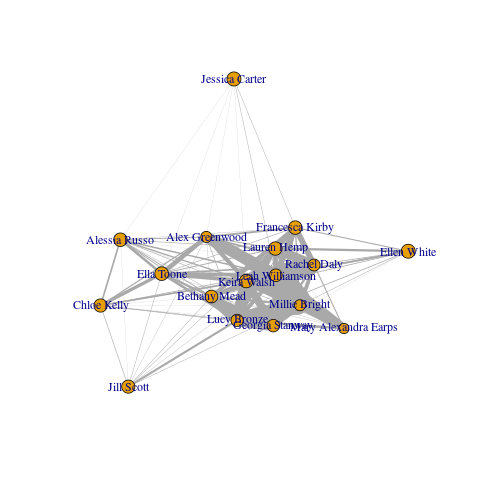
\includegraphics[width=\textwidth]{./img/plot_england_simpl.png}
   \caption{Red de pases total de Inglaterra simplificado en la EURO 2022}
   \label{img:red:simpl:eng}
\end{figure}

En \ref{img:ent:eng} estudiamos cómo es consistente con lo ya comentado, y hay poca variabilidad dentro de la 
entropía, conteniendo únicamente extremos mínimos correspondientes a la portera y máximos correspondientes a las defensas. 
Nos reafirma en que la entropía refleja bien el comportamiento en el campo, la posición de las jugadoras y cuántos 
minutos jugaron.

\begin{figure}[h!tbp]
  \centering
   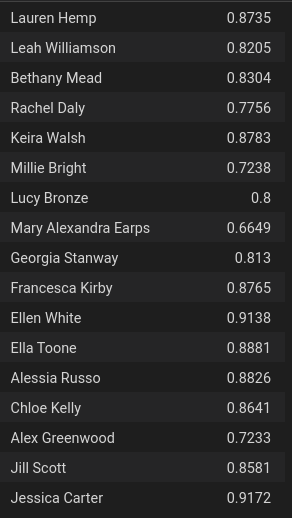
\includegraphics[width=\textwidth]{./img/entrop_engl.png}
   \caption{Entropía por jugadoras de Inglaterra en la EURO 2022}
   \label{img:ent:eng}
\end{figure}

En \ref{img:red:eng} vemos las redes de peso sin simplicar las aristas, lo que nos permite apreciar lo densa que es, pero a su 
vez están bien repartidas, y no apelotonadas como en Noruega \ref{img:red:norw}.

\begin{figure}[h!tbp]
  \centering
   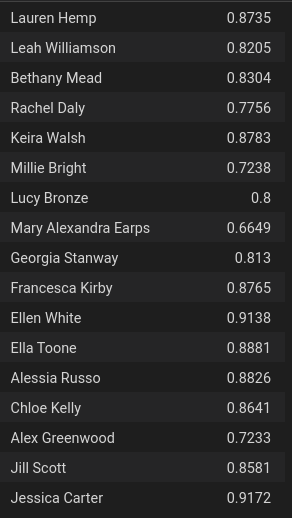
\includegraphics[width=\textwidth]{./img/entrop_engl.png}
   \caption{Entropía por jugadoras de Inglaterra en la EURO 2022}
   \label{img:red:eng}
\end{figure}

En \ref{img:red:simpl:nor} y \ref{img:red:nor} vemos que no es tanto una estructura casi romboidal, sino circular; 
están más juntas y sin una forma reticular clara.

\begin{figure}[h!tbp]
  \centering
   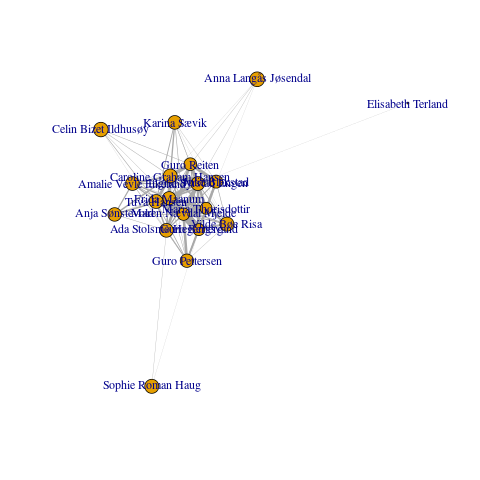
\includegraphics[width=\textwidth]{./img/plot_norw_simpl.png}
   \caption{Red de pases total simplificado de Noruega en la EURO 2022}
   \label{img:red:simpl:nor}
\end{figure}

\begin{figure}[h!tbp]
    \centering
     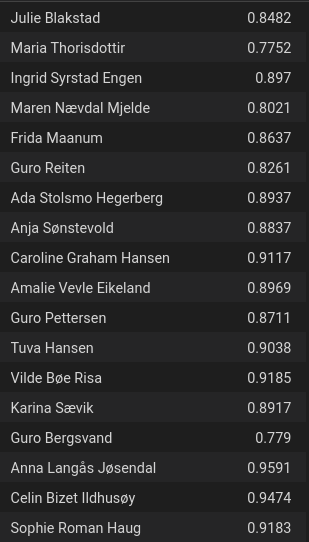
\includegraphics[width=\textwidth]{./img/entrop_norw.png}
     \caption{Entropía por jugadoras de Noruega en la EURO 2022}
     \label{img:red:nor}
\end{figure}

\begin{figure}[h!tbp]
    \centering
     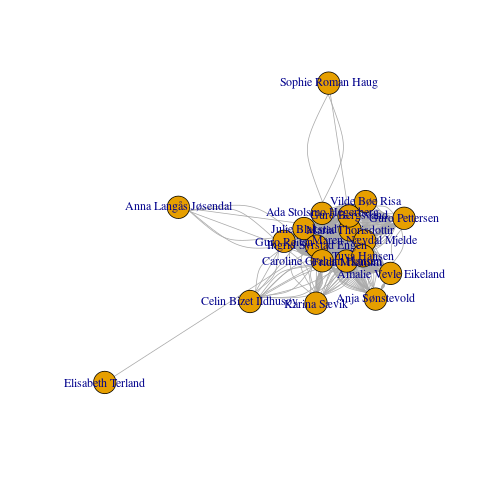
\includegraphics[width=\textwidth]{./img/plot_norw.png}
     \caption{Red de pases total de Noruega en la EURO 2022}
     \label{img:ent:norw}
\end{figure}

En \ref{img:fineng} y \ref{img:finnorw} vemos cómo Noruega se mantuvo con una entropía bastante alta en general
(lo que podemos ver reflejado en\ref{img:ent:norw}), 
mientras que la de Inglaterra es una curva decreciente, por lo que tienen orden y desorden, y consiguen un buen 
equilibrio.

\begin{figure}[h!tbp]
    \centering
     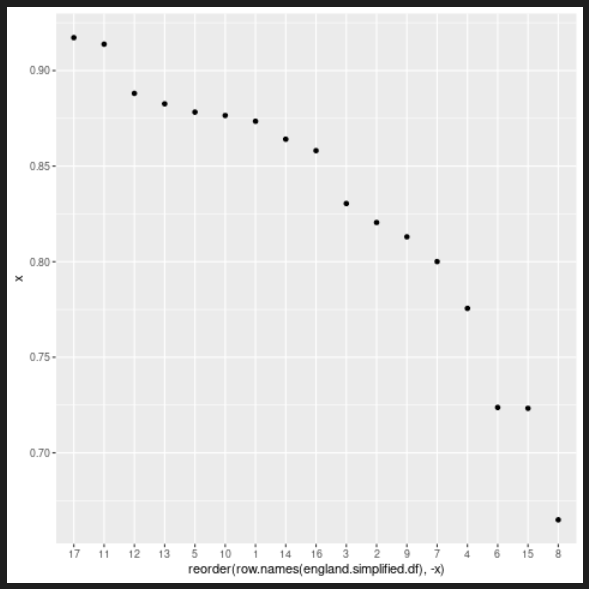
\includegraphics[width=\textwidth]{./img/englandentropy.png}
     \caption{Entropía de Inglaterra}
     \label{img:fineng}
\end{figure}

\begin{figure}[h!tbp]
    \centering
     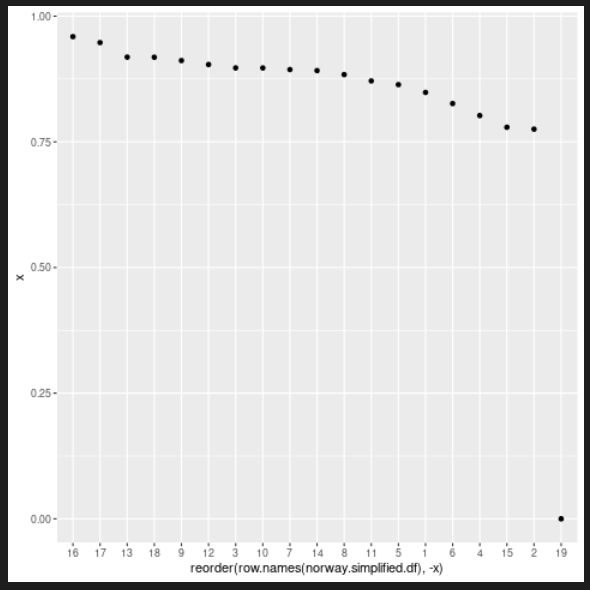
\includegraphics[width=\textwidth]{./img/norwayentrop.png}
     \caption{Entropía de Noruega}
     \label{img:finnorw}
\end{figure}

\section{Costes}
En cuanto a coste de amortización anuales, he usado mi portátil Asus Vivobook 14, comprado hace casi tres 
años por 799€, lo que se corresponde a 150€. El coste de desarrollo, teniendo en cuenta que 
hemos empleado 571 horas, entre 40 que son las horas que se echan por semana en un trabajo a 
tiempo completo, nos quedamos con 14 semanas, esto es, unos tres meses y medio. Si consultamos 
\href{https://www.linkedin.com/feed/}{LinkedIn}, las ofertas de trabajo para desarrolladores 
\textit{junior} están en torno a los 21.000€ al año, lo que viene a ser 1750€ por mes, añadiendo los 14€ 
que costaron el ventilador de Alehop mencionado en los agradecimientos. Esto se
muestra en la tabla \ref{tab:costes1}

\begin{table}
\begin{tabular}[h!tbp]{lccr}
  Concepto & Coste unitario & Unidades & Total \\
  Amortización portátil & 150€ & 1 & 150€ \\
  Ventilador            & 12€  & 1 & 14€ \\
  Costes laborales      & 1750€& 3.5 & 6125€ \\
  \hline \\
  \multicolumn{3}{l}{Total} & 6289€ \\
\end{tabular}
\caption{Costes el proyecto en el escenario ``ingeniera junior''} \label{tab:costes1}
\end{table}

Sin embargo, el trabajo realizado aquí corresponde más bien al de un analista
junior de datos deportivos. Según \href{https://www.payscale.com/}{Payscale}, el sueldo medio está en torno 
a los24000€. En este escenario los costes serían los indicados en la tabla \ref{tab:costes2}.

\begin{table}
\begin{tabular}[h!tbp]{lccr}
  Concepto & Coste unitario & Unidades & Total \\
  Amortización portátil & 150€ & 1 & 150€ \\
  Ventilador            & 12€  & 1 & 14€ \\
  Costes laborales      & 2000€& 3.5 & 7000€ \\
  \hline \\
  \multicolumn{3}{l}{Total} & 7164€ \\
\end{tabular}
\caption{Costes el proyecto en el escenario ``analista de datos junior''} \label{tab:costes2}
\end{table}

El coste de explotación, despliegue y producción se corresponderán a servicios de 
desarrollo a medida, adaptación, implantación, cursos, entre otros, pero este
tipo de trabajos se suelen hacer en nómina o bien vendiendo los informes; el
coste del informe trataría de ponerse de acorde con las horas empleadas y la
amortización del equipo durante el tiempo necesario. Una vez llevado a cabo todo
el análisis inicial y la exploración de los métodos, la elaboración de un nuevo
informe de este tipo se estima que duraría unos 15 días.

La biblioteca tendremos que 
mirarla cada cierto tiempo, actualizar dependencias, responder a los issues, para lo que echaremos 
40 horas al mes, que serán costes de producción que tendremos que factorizar en el coste del producto.
